\title{Type-Safe Covariance in \CC{}}
\author{
        %\large
        \textsc{Vitaly Surazhsky}
            \qquad
        \textsc{Joseph (Yossi) Gil}\thanks{Contact author}
        \mbox{}\\ %
        Department of Computer Science\\
        Technion---Israel Institute of Technology\\
        Technion City, Haifa 32000, \underline{Israel}\\
        \mbox{}\\ %
        \normalsize
            \texttt{vitus}
        \textbar{}
            \texttt{yogi}
        \normalsize
            \texttt{@cs.technion.ac.il}
}
\date{\today}
\documentclass[11pt]{article}
%\documentclass{acmconf}

\usepackage[paper=a4paper,dvips,top=1.5cm,left=1.5cm,right=1.5cm,
    foot=1cm,bottom=1.5cm]{geometry}

\usepackage{times}
%\usepackage{graphicx}
\usepackage[fleqn]{amsmath}
\usepackage{amsfonts}
\usepackage{amssymb}
\usepackage{amsthm}
\usepackage{amsopn}
\usepackage{xspace}
\usepackage{array}
\usepackage{epsfig}

\numberwithin{figure}{section}

\newcommand\CC{\Lang{\mbox{C++}}\xspace}
\newcommand\Lang[1]{\textsc{#1}}
\newcommand{\kw}[1]{\texttt{\textbf{#1}}}
\newcommand{\cd}[1]{\texttt{#1}}

\newcommand\Naturals{\ensuremath{\mathbb{N}}\xspace}
\newcommand\Integers{\ensuremath{\mathbb{Z}}\xspace}
\newcommand\Rationals{\ensuremath{\mathbb{Q}}\xspace}
\newcommand\Reals{\ensuremath{\mathbb{R}}\xspace}
\newcommand\Complex{\ensuremath{\mathbb{C}}\xspace}

\newcommand\norm[1]{\ensuremath{\lVert#1\rVert}}
\newcommand\abs[1]{\ensuremath{\lvert#1\rvert}}
\newcommand\ceil[1]{\ensuremath{\lceil#1\rceil}}
\newcommand\floor[1]{\ensuremath{\lfloor#1\rfloor}}
\newcommand\set[1]{\ensuremath{\{#1\}}}
\newcommand\angular[1]{\ensuremath{\langle#1\rangle}}

\newcommand\Norm[1]{\ensuremath{\left\lVert#1\right\rVert}}
\newcommand\Abs[1]{\ensuremath{\left\lvert#1\right\rvert}}
\newcommand\Ceil[1]{\ensuremath{\left\lceil#1\right\rceil}}
\newcommand\Floor[1]{\ensuremath{\left\lfloor#1\right\rfloor}}
\newcommand\Set[1]{\ensuremath{\left\{#1\right\}}}
\newcommand\Angular[1]{\ensuremath{\left\langle#1\right\rangle}}

\newcommand{\LOOM}{\ensuremath{\cal{LOOM}}\xspace}
\newcommand{\PolyTOIL}{\textbf{PolyTOIL}\xspace}

\newtheorem{theorem}{Theorem}[section]
\newtheorem{definition}[theorem]{Definition}
\newtheorem{lemma}[theorem]{Lemma}
\newtheorem{corollary}[theorem]{Corollary}
\newtheorem{fact}[theorem]{Fact}
\newtheorem{example}[theorem]{Example}

\newcommand\Cls[1]{\textsf{#1}}
\newcommand\Fig[1]{Figure~\ref{Figure:#1}}

\usepackage{labels} %
\usepackage{equation}
\usepackage{prog2tex}

\newenvironment{excerpt}{\begin{quote}\begin{minipage}\textwidth}{\end{minipage}\end{quote}}

\setcounter{topnumber}{0}
\setcounter{bottomnumber}{0}
\setcounter{totalnumber}{20}
\renewcommand{\textfraction}{0.01}

\begin{document}

\maketitle

\begin{abstract}
We present a programming technique for implementing
    type safe covariance in \CC{}.
In a sense, we implement most of Bruce's \emph{matching}
    approach to the covariance dilemma in \CC.
The appeal in our approach is that it relies on existing mechanisms,
    specifically templates, and does not require any
    modification to the existing language.
The practical value of the technique was demonstrated
    in its successful incorporation in a large software body.
We identify the ingredients of a programming language
    required for applying the technique, and discuss
    extensions to other languages.
\end{abstract}

\section{Introduction}
Two clashing forces make
    the recalcitrant covariance dilemma.
On the one hand, virtually all modeling situations
    are \emph{covariant} in nature, i.e., a specialization in
    one hierarchy
    is correlated with a specialization
    in another hierarchy.
A problem-world example is the \Cls{child} specialization of a
    \Cls{person}, which is correlated with a specialization
    of \Cls{physician} to a \Cls{pediatrician}.
A program-world example is the specialization of
    \Cls{singly-linked-list} into \Cls{doubly-linked-list},
    correlated with the specialization of \Cls{singly-linked-node}
    into \Cls{doubly-linked-node}.
Famous are also cases of \emph{auto-covariance} in which changes
    a hierarchy is correlated with itself.
For example, comparing instances of \Cls{point} for equality is specialized
    into comparing instances of \Cls{color-point}.

On the other hand, it is impossible to statically
    type-check inclusion polymorphism~\cite{Cardelli:Wegner:85}
    when covariance is allowed.
Suppose for example that instances of \Cls{child}
    can be freely used at any place where instances of \Cls{person}
    might.
Then, one of these places, might associate
    a certain \Cls{physician} who is not
    a \Cls{pediatrician} with a \Cls{child}.
Such an association can only be prevented with run-time
    type checks.
(For a more detailed exposition of covariance see sections 3--4 in Kim Bruce's
    lecture notes~\footnote{\texttt{http://www.cs.williams.edu/\textasciitilde kim/README.html\#Static}}
    on the topic.)

In dealing with this dilemma, different programming languages in practical
    use take different approaches.
Favoring modeling convenience
    language such \Lang{Smalltalk}~\cite{Goldberg:Robson:Book:83}
    and \Lang{CLOS}~\cite{Steele:90} do not impose static type checking.
Favoring static typing over modeling convenience some languages,
    such as early versions of \CC~\cite{Stroustrup:Book:91},
    forbid covariance altogether.
Other languages allow it a restricted form.
For example, current \CC~\cite{Stroustrup:Book:97} permits
    covariant changes only to function return type, since this can
    be statically checked.
\Lang{Sather}~\cite{Szypersky:Omohundro:Murer:93,Omohundro:94} extends this by allowing
    \emph{contravariant} changes to arguments, which is not
    very useful for modeling, but can be statically checked.


A combination of static and dynamic checks can also be found.
In the \Lang{Java}~\cite{Arnold:Gosling:96} case, even though
    covariance cannot be declared or statically checked,
    it is possible for a programmer to use a downcast
    relying on a covariance presumption.
The runtime system will then detect all type errors
    resulting from making this assumption.
\textsc{Eiffel}~\cite{Meyer:Eiffel:92} is unique in allowing
    covariant definitions, using what is called \emph{anchored types}.
Type safety is then achieved by a link-time dataflow analysis,
    known as ``system validity check''.
Apparently, system validity check was never part
    of commercial \Lang{Eiffel} compilers, which
    therefore compromise static type safety.

Virtual types in
    \Lang{Beta}~\cite{Madsen:Moller-Pedersen:Nygaard:93}
    are yet another form of covariance.
Even though \Lang{Beta} is in general type safe,
    the type correctness of those aspects of the language
    which touch virtual types are is ensured by runtime checks.

In summary, none of these languages succeeds in combining
    type safety and the convenience of covariant modeling.

Stepping beyond current languages, type theorists dedicated
    much attention to the problem.
The exact types approach~\cite{Bruce:97} restricts covariance
    as follows.
In each call of the form
\beq{poly}
    c.m(d)
\eeq
it is required that if~$m$ is covariantly overridden,
        either~$c$ must be of an \emph{exact type}~$C_1$, i.e., it is not
        allowed to be of any type~$C_2 \prec C_1$,~$C_2 \ne C_1$.
Meyer's polymorphic
    catcalls~\footnote{\texttt{http://www.eiffel.com/doc/manuals/technology/typing/cat.html}}
    are a variation in which dataflow analysis replaces an exact type declaration
    in guaranteeing that~$c$ is monomorphic.
An experimental implementation of exact types was in \Lang{Eiffel}
    recently
    reported~\cite{Colnet:Liquori:00}.

Catagana~\cite{Castagna:95} on the other hand
    convincingly argued for \emph{encapsulated multi-methods} in which
    the polymorphic nature of~\eq{poly} is enriched
    rather than restricted.
Consider a definition of a method $m$ in class $C_1$,
\beq{original}
    m(a:D_1) = \ldots
\eeq
with a covariant definition in class $C_2 \prec C_1$
\beq{override}
    m(a:D_2) = \ldots
\eeq
where $D_2 \prec D_1$.
Then, definition~\eq{override} \emph{adds}
    to~\eq{original}, rather than merely
    overriding it.
The polymorphic call~\eq{poly} is implemented
    as a \emph{multi-dispatch}:
    if $c \in C_2$ \emph{and}~$d \in D_2$,
        then the implementation~\eq{override} is invoked.
Otherwise, the implementation~\eq{original} is used.
Multi-methods support subtyping, static typing and covariance,
    at the price of deviating from the single-dispatch tradition
    of object oriented languages.
Also, multi-methods do not support covariant changes to field
    types.

Problems such as type-checking~\cite{Chambers:Leavens:95},
    and especially in a separate
    compilation environment~\cite{Millstein:Chmabers:99}, compounded
    by the non-OO semantics, are most likely the reason
    that multi-methods did not yet find their way into
    mainstream programming languages.
The \textsc{Visitor} pattern~\cite{Gamma:Helm:Johnson:Vlissides:Book:95} in its many
    incarnations is nothing but
    a programming technique for implementing multi-methods in
    single-dispatch languages.

\emph{Matching}, the other major
    type-theoretical approach, resolves the covariance dilemma
    by slightly weakening the notion of subtyping and
    somewhat restricting runtime substitutability.
Matching was demonstrated in research languages
    such as \PolyTOIL~\cite{Bruce:Fiech:Schuett:vanGent:95},
    \LOOM~\cite{Bruce:Fiech:Petersen:97} and
    LGM~\cite{Rinat:00}.
Matching is a weaker notion than
    the subtyping in the sense that if a type
    matches another, then it cannot be substituted freely
    for it.
Covariant specialization is on the other hand allowed
    along the matching relationship.
With matching, inclusion polymorphism gives
    way to \emph{match bounded polymorphism} which dwells on the notion
    of \emph{match type}, the type of all entities of
    of types matching a certain type.

The contribution in this paper is a programming
    technique for implementing matching
    statically typed contemporary languages,
    specifically \CC, without any modification
    to the language syntax and semantics.
Our type safe implementation is used
    successfully in a large application for
    managing geometrical and graph theoretical
    entities.

The techniques uses familiar programming techniques,
    specifically template programming similar, but
    of a smaller scale than STL~\cite{Musser:Saini:96}
    or compile time symbolic derivation~\cite{Gil:Gutterman:98}.
We therefore believe that the technique would be appealing
    to some programmers than the more theoretical advances.
After learning the basic notions, the programmer
    essentially in \CC{}.

Also worthy of notice is that the technique combines
    the flexibility advantage of dynamic typing with
    the safety of static typing.
The flexibility and the convenience of using the technique
    comes from the fact that the programmer does not have
    to define or understand sophisticated type declarations,
    drawn from a rich and powerful type system.
However, since the technique used templates and template
    expansion, the body of computation is carried out
    at compile time.
``type errors'' will result in the production of compiler error messages,
    and in failure to generate the covariant classes.
Hence, the programmer is saved the trouble of making a
    type correct mutual covariant definition of a matching hierarchy
    base, which should guarantee that all descendants
    of a certain type are type correct.
Instead, the programmer tries to define each
    class in the hierarchy in its turn.
It is not guaranteed that each class defined will
    be type correct.
Each such class will ingratiate some templates.
``Run time'' type errors, as a result our lack to ability
    the sophisticated type system, will make ``run time'' errors.
However, since template expansion is at compile time, these
    errors will be emitted by the compiler, as compiler errors.



\paragraph{Outline}
\Ref{Section}{simple} uses the example of a covariant graph hierarchy to introduce
    the concept of configuration classes, and the way they are used in the implementation.
To make a smooth discourse, the presentation uses at this stage several
    \CC macros, designed to hide some of the \CC lingo.
We then continue in \Ref{Section}{special}
    to discuss auto covariance, and in comparing our technique with \LOOM.
In \Ref{Section}{recursive} reviews the two examples from a more programming language
    theoretical perspective.
In particular, this section discusses the notions of recursive
    and collateral definitions, and the way their realization
    in \CC makes our solution possible.
\Ref{Section}{recursive} also reveals the \CC{} macros used
    in \Ref{Section}{simple}.
In the final \Ref{Section}{Conclusions} we discuss the results, trying
    to explain concludes the paper with
    some directions for future research.

\Section[simple]{A Covariant Graph Hierarchy Example}
In this section, we give a quick introduction to our solution
    of the covariance dilemma, showing how it might be used by a \CC programmer.
For the purpose of exposition some of the intricate details are hidden
    behind \texttt{\#define} macros.
The fine details will be revealed in \Ref{Section}{recursive}.

Most examples in the literature revolve around the theme of auto-covariance,
    such as a class \Cls{Point} with an \Cls{equal} method,
    specialized by \Cls{ColorPoint}.
We will start with the more general case, as
    illustrated in \Ref{Figure}{Graphs}.

\begin{figure}[!htb] % Graphs
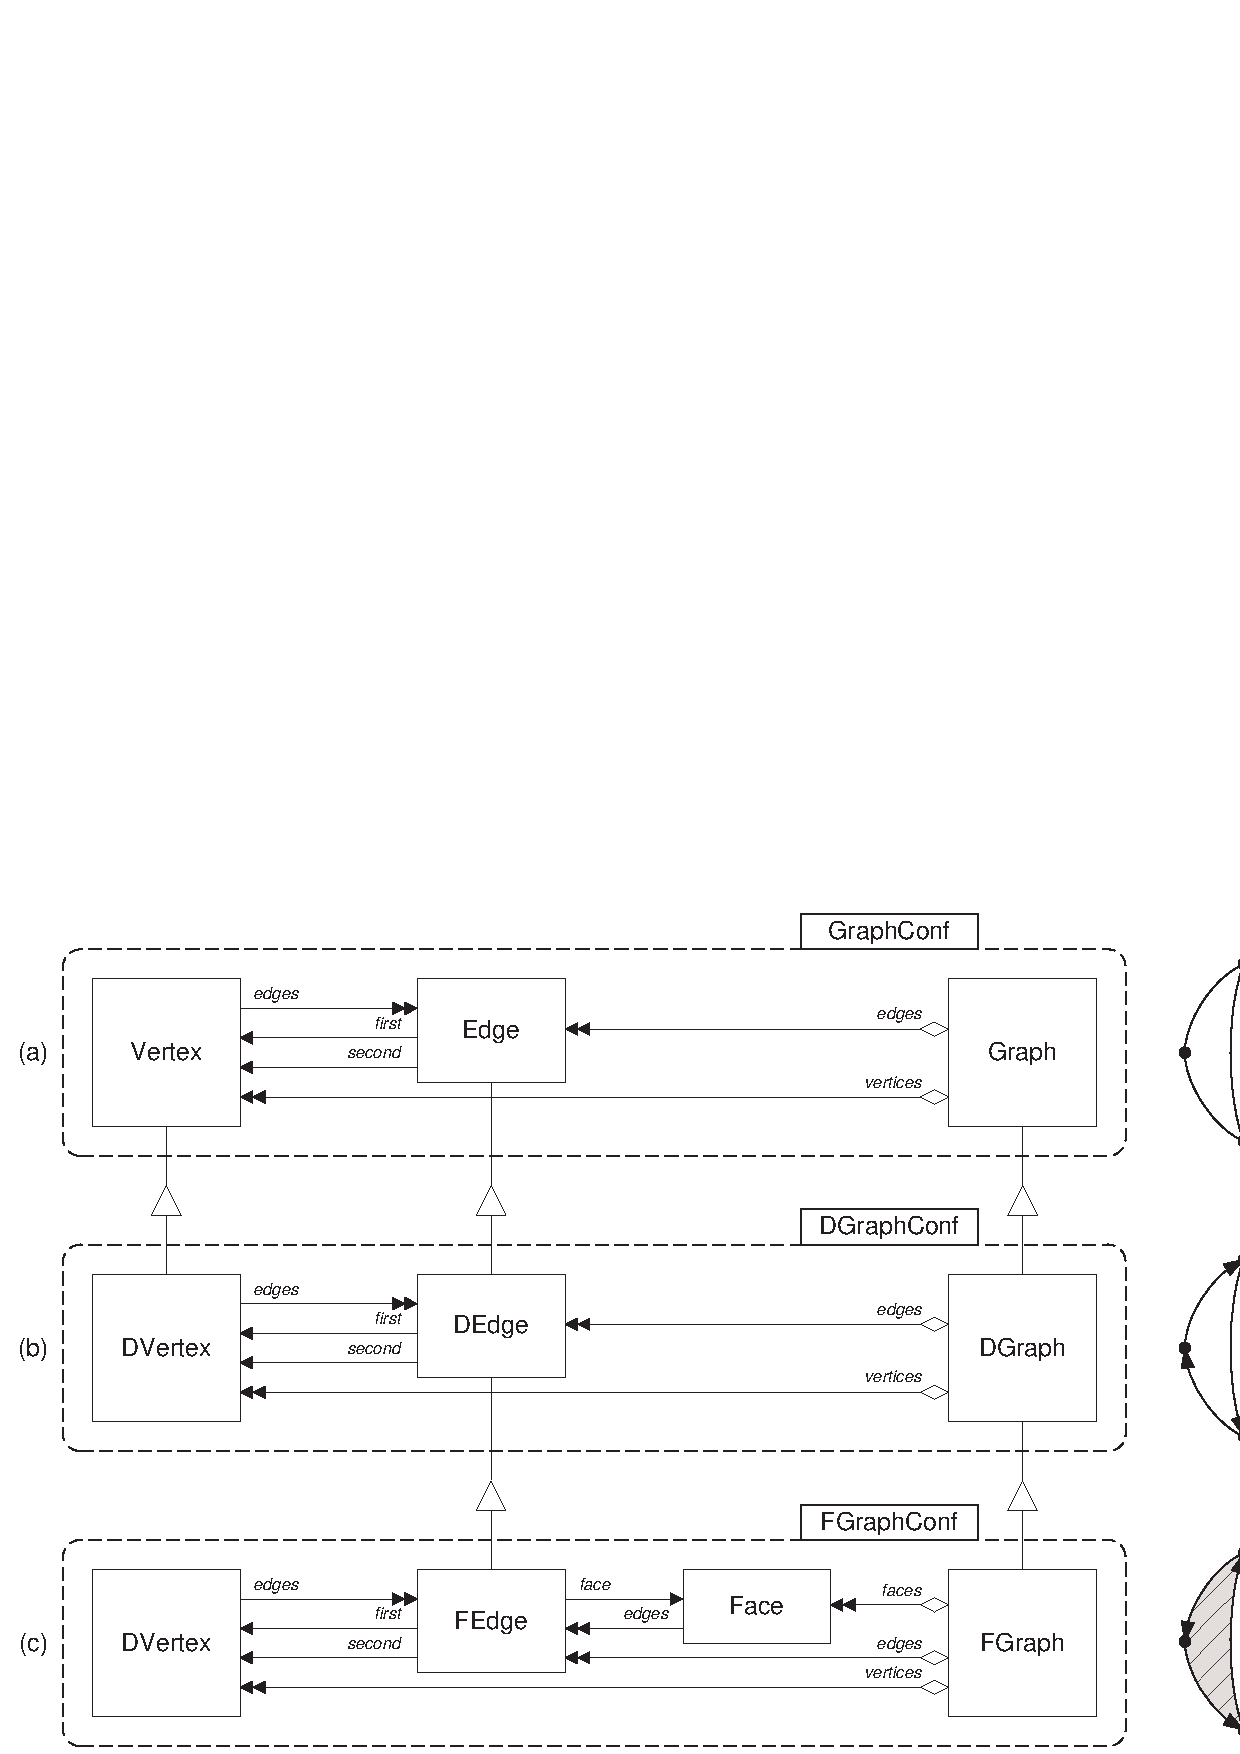
\includegraphics[width=\textwidth]{graphs.pdf}
\caption{The Graphs diagrams}
\label{Figure:Graphs}
\end{figure}

The figure illustrates a covariant hierarchy
    modeling various entities in graph theory.
The hierarchy is drawn from a 10KLOC \CC library
    of algorithms of 2D shape morphing in computer
    graphics~\cite{Gotsman:Surazhsky:01}.%
\footnote{We hope that this real-life example is more appealing to our programming
    intuition than \Cls{Animal}-\Cls{Hebivore}-\Cls{Dish}-\Cls{Food} sort
    of examples sometimes used in the literature.
There is no fundamental between the two.}
The two classes \Cls{Vertex} and \Cls{Edge} comprise
    a graph from the graph theory and describe the basic behavior and functionality.

At the top of the figure (a) we see that a \Cls{Graph} has a set of instances of \Cls{Edge}
    and a set of instances \Cls{Vertex}.
Each \Cls{Edge} has two references (\Cls{first} and \Cls{second}) to vertices.
A \Cls{Vertex} has a list of references to the edges incident on it.
At the middle section (b) of the figure, we see that \Cls{DGraph} modeling
    a directed graph, specializes \Cls{Graph}.
A directed graph has directed edges, and directed vertices.
Thus, \Cls{DVertex} and \Cls{DEdge} specialize \Cls{Vertex} and
    \Cls{DEdge} respectively.

The bottom section~(c) of the figure models the concept of \emph{face graph},
    which is a directed planar graphs augmented with face information.
A \emph{face} is a cyclic sequence of edges forming
    a simple cycle in a graph.
Intuitively, an embedding of a planar graph in the plane
    subdivides the plane into regions.
Each region is represented by a face, which also defines an
    order for traversing the edges surrounding it.
The specialization of \Cls{DGraph} in \Cls{FGraph} is correlated
    with a specialization of \Cls{DEdge} into \Cls{FEdge}.
Note that \Cls{FEdge} stores a reference to \Cls{Face}---a new concept
    which does not exists in directed graphs.


\Ref{Figure}{Graph} shows the definitions for the face graph.
Class \Cls{FGraph} being derived from \Cls{DGraph} holds objects
    of vertices, edges and faces, and extends the functionality of class \Cls{DGraph}.
The vertices of the face graph has the same behavior and structure as those
    of the directed graph except for the type of its adjacent edges.
The configuration definition of the face graph reflects the usage of class \Cls{DVertex}
    in the arrangement of the face graph classes.
Instances of type \Cls{FGraph} and of type \Cls{Face} are created to demonstrate
    the usage of the definitions.

The \CC implementation of \Ref{Figure}{Graphs}
    is presented in figures~\ref{Figure:Graph}--\ref{Figure:FGraph}.


In implementing covariance, the programmer must be thinking
    in terms of actors, roles, and configurations.
The three concepts are not supported as such in \CC,
    hence the use of macros, which are all written in all capitals.
An actor may interact with roles, and assume other roles.
Actors may be specialized.
Covariance specialization of an actor is realized
    by changing the actors which assume the roles
    with which this actor interacts.
(Later we will see that actors nothing but are generic classes, or
    class templates as they are known in the \CC jargon.)

\Ref{Figure}{Graph} illustrates the definition of actors.

\begin{figure}[!htb]
\CPP
ACTOR Edge { public:
    INTERACTS_WITH(V);
    Edge(V& v1, V& v2);            // a covariant constructor
    void set_first(V* v);          // a covariant method
    void set_second(V* v);         // another covariant method
    V& get_first();                // a method with a covariant return value
    //{} more definitions \ldots
    protected: V *first, *second;  // two covariant fields
};
ACTOR Vertex { public:
    INTERACTS_WITH(E);
    void insert_edge(E *e);        // a covariant method
    void delete_edge(E *e);        // another covariant method
    //{} \ldots
    protected: list<E *> edges;    // a covariant field
};
ACTOR Graph { public:
    INTERACTS_WITH(V);
    INTERACTS_WITH(E);
    Graph(list<V *>& vs, list<E *>& es);   // a doubly covariant constructor
    //{} \ldots
    protected: list<V *> vertices; list<E *> edges;
};
\END\PROGb{}
\caption{The actors of an undirected graph}
\label{Figure:Graph}
\end{figure} % Graph

Three actors: \cd{Edge}, \cd{Vertex} and \cd{Graph}
    are defined in the figure.
If the type of an field, a method argument, or function return value
    in an actor may take covariant specialization, then
    this type must be declared as a \emph{role}.
(Later we will see that roles are realized as
    \kw{typedef}s in a class passed as an argument to the
    class template which realizes an actor.)
A definition of an actor starts with a series of
    \cd{INTERACTS\_WITH} directives,
    each declaring a role with which the actor may interact.
There are three roles with which the actors in \Ref{Figure}{Graph} interact:
    \cd{G} designating graphs, \cd{V} designating vertices,
    and \cd{E} designating edges.
Actor \cd{Graph}, for example, interacts
    with roles \cd{V} and \cd{E}.

Other than stating that a role is a type,
    the role declaration does not place any explicit
    constraints on it.
Once the interacting roles are defined,
    the definition of an actor is similar
    to a \CC class definition, where roles can
    be used anywhere types are used.
For example, actor \cd{Edge} has a covariant constructor taking two arguments
    whose type is the role \cd{E}, methods \cd{set\_first} and \cd{set\_second}
    each taking a covariant argument, a method \cd{get\_first} with
    a covariant return type, two covariant field definition (\cd{first}
    and \cd{next}), and possibly more covariant and nonvariant member definitions.

The body of an actor may, and usually will, place
    implicit constraints  on the roles it interacts with.
In the figure, actor \cd{Edge} makes the
    assumption that type \cd{V} is such that
    both \cd{V *} and \cd{V \&} are valid types.
This assumption does not hold for example for the
    type \cd{int \&}.
More interesting assumptions on \cd{V} are made by, say,  the body of the method
    \cd{set\_first(V)}:
\begin{quote}
\begin{minipage}{\textwidth}
\CPP
    set_first(V* v)
    {
        if (first != 0)
            first->delete_edge(this);
        first = v;
        v->insert_edge(this)
    }
\END\PROGc{}
\end{minipage}
\end{quote}
It is assumed in the above code excerpt that
    role \cd{V} has two methods named \cd{delete\_edge}
    and \cd{insert\_edge}
    which can receive a parameter of the type of \kw{this}.
For a set of actors $A$ which interact with a set of roles $R$,
    let $c(A)$ be the set of assumptions that $A$ makes on $R$.%
\footnote{
    The definition of set $c(A)$ is deliberately very loose.
We do not state what assumptions might be there,
    how they are structured, etc.}

Actors are made into concrete classes, and used to
    instantiate objects, only after roles are assigned to them.
A \emph{configuration} is
    a simultaneous assignment of roles to actors,
    creating a set of cooperating classes.
(Later we will see that configurations are realized
    as a series of \kw{typedef}s made in a class
    passed as a template parameter to an actor.)

Mathematically, a configuration is a mapping
    the set $R$ of roles onto the set $A$ of actors,
    such that each role is assigned to exactly one
    actor.
An actor may however may assume more than one role.
The assignment must be consistent in the sense
    that the set of constraints $c(A)$ must hold
    for the set of role-actor pairs.

Consider for example the
    configuration of undirected graphs, as illustrated
    in \Ref{Figure}{undirected:configuration}.

\begin{figure}[!htb]
\begin{minipage}[t]{0.5\textwidth}
\CPP
CONFIGURATION(GraphConfig)
    ASSIGN_ROLE(V, Vertex)
    ASSIGN_ROLE(E, Edge)
    ASSIGN_ROLE(G, Graph)
END_CONFIGURATION
\END\PROGd{}%
\end{minipage}%
\caption{A configuration of an undirected graph}
\label{Figure:undirected:configuration}
\end{figure}


Configuration \cd{GraphConfig}
    assigns the roles \cd{V} (a vertex) \cd{E} (an edge)
        and \cd{G} (a graph)
        respectively to actors \cd{Vertex}, \cd{Edge} and \cd{Graph}.
The above role assignment does a \emph{simultaneous} substitution
    in \Ref{Figure}{Graph}, to create three ordinary \CC class,
    out of which objects can be instantiated as in \Ref{Figure}{directed:objects}.



\begin{figure}[!htb]
\begin{minipage}[t]{0.5\textwidth}
\CPP
GraphConfig::V v1, v2, v3;
GraphConfig::E e12(v1,v2), e23(v2, v3);
GraphConfig::G g(CONS(&v1,CONS(&v2, &v3)), CONS(&e12, &e23));
\END\PROGe{}%
\end{minipage}%
\caption{Instantiating the \cd{GraphConfig} configuration}
\label{Figure:directed:objects}
\end{figure}

As we can see in the figure,
    selecting a certain role out of a configuration
    is done simply by using the \cd{::} operator.
Trying to elicit roles from a configuration in which
    they are not defined, will result in a compiler error.
Similarly, a configuration which does not create a complete
    or consistent role assignment, will result in a compiler error.
In general, these errors may not be easy to understand.

In the figure, we construct three
    directed vertices, \cd{v1}, \cd{v2}, and \cd{v3},
    and edges \cd{e12} (connecting \cd{v1} to \cd{v2})
    and \cd{e23} (connecting \cd{v2} to \cd{v3}).
The directed graph \cd{g} is then constructed with the two lists $(\cd{v1}, \cd{v2})$
    and $(\cd{e1}, \cd{e2}, \cd{e3})$.
A \Lang{Lisp}-like \cd{CONS} function
    is used for creating the lists.
The implementation of \cd{CONS} is standard using an overloaded
    template function, and will not be repeated here.

\Ref{Figure}{directed:objects} helps also
    understand the circular nature of the substitution in a configuration.
The \CC class \cd{GraphConfig::V} is in fact the
    actor \cd{Vertex}, with the role \cd{E} substituted by
    the \CC class \cd{GraphConfig::E}.
The \CC class \cd{GraphConfig::E} is in its turn
    obtained by substituting the role \cd{V} by the \CC class \cd{GraphConfig::V}
        in actor \cd{Edge}.
The \CC class \cd{GraphConfig::G} is obtained
    by making both these role substitutions in
    actor \cd{Graph}.
The definition of these three \CC classes
    is mutually recursive.

The configuration \cd{GraphConfig} is consistent since
    actor \cd{Edge} indeed has
    two functions named \cd{delete\_edge} and \cd{insert\_edge}.
The assumption about the type of the arguments is satisfied by the
    class \cd{GraphConfig::V}, in which the arguments to
    \cd{delete\_edge} and \cd{insert\_edge} are of type
    \cd{GraphConfig::E}.


Circular definitions exist as such in \CC{}.
The main purpose of the distinction between actors and roles is that
    new actors can be specialized from existing actors,
    inheriting the roles they interact with.
An example of actor specialization is given in \Ref{Figure}{DGraph},
    where actor \cd{DEdge} specializes \cd{Edge} etc.

\begin{figure}[!htb]
\CPP
SPECIALIZED_ACTOR(DEdge, Edge) { public:
    //{} role \cd{V} is inherited
    V* source() const; V* target() const;
    // more functionality
    protected: //  new internal staff
};
SPECIALIZED_ACTOR(DVertex, Vertex) { public:
    //{} role \cd{E} is inherited
    //{} extend functionality \ldots
    protected: // new internal staff
};
SPECIALIZED_ACTOR(DGraph, Graph) { public:
    //{} roles \cd{V} and \cd{E} are inherited
    //{} new functionality and algorithms
    protected: // new internal staff
};
\END\PROGf{}
\caption{The actors in a directed graph}
\label{Figure:DGraph}
\end{figure} % DGraph

The macro \cd{SPECIALIZED\_ACTOR} creates
    a new actor specializing an existing one.
Actor specialization is just
    like derivation in \CC, and the specializing
    actor can override the definitions in the specialized
    actor, adding to them, etc.
However, since actors are not classes,
    a derived actor cannot be used where
    the base actor is used.
Hence the covariance dilemma does not appear.

Since no constraints are placed on roles,
    it is not necessary to change the definition
    the role in a derived class.
The triple of covariant classes realizing the directed graph
    concept is realized by a configuration
    assigning respective roles the three actors, as done
    by \Ref{Figure}{directed:configuration}.
Again, the configuration \cd{DGraphConfig} in this figure
    does a simultaneous substitution, this time on the actors
    defined in \Ref{Figure}{DGraph}.
Three new \CC classes \cd{DGraphConfig::E}, \cd{DGraphConfig::V},
    and \cd{DGraphConfig::G},
    are generated from the three actors, by a consistent substituting of the
    roles with the newly generated classes.

Again, the definition of these three
    new classes is mutually recursive.
The \emph{structure} of this mutual recursion is similar to that
    of of the mutual recursion in the three classes generated
    by configuration \cd{GraphConfig}.
However, the class \cd{DGraphConfig::V}
    (say) does not inherit from the class \cd{GraphConfig::V},
    even though these two classes were defined
    using the same role assigned to two actors bounded
    together by specialization.

\begin{figure}[!htb]
\begin{minipage}[t]{0.5\textwidth}
\CPP
CONFIGURATION(DGraphConfig)
    ASSIGN_ROLE(V, DVertex)
    ASSIGN_ROLE(E, DEdge)
    ASSIGN_ROLE(G, DGraph)
END_CONFIGURATION
\END\PROGg{}%
\end{minipage}%
\caption{A configuration of a directed graph}
\label{Figure:directed:configuration}
\end{figure}

A faced graph requires yet another actor \cd{Face}.
The complete definition of the actors in face graph is
    given in \Ref{Figure}{FGraph}.
Actor \cd{Face} interacts with edges (role \cd{E}),
    and stores a list of edges.

\begin{figure}[!htb]
\CPP
SPECIALIZED_ACTOR(FEdge, DEdge) { public:
    //{} role \cd{V} is inherited
    INTERACTS_WITH(F);
    F* getFace() const { return face; }
    // more functionality
    protected:  F* face;
};
ACTOR Face { public:
    INTERACTS_WITH(E);
    //{} \ldots
    protected: list<E*> edges;
};
SPECIALIZED_ACTOR(FGraph, DGraph) { public:
    INTERACTS_WITH(F);     //{} roles \cd{V} and \cd{E} are inherited
    //{} \ldots
    protected: list<F*> faces;
};
\END\PROGh{}
\caption{The actors in a face graph}
\label{Figure:FGraph}
\end{figure} % FGraph

Note that we do not specialize the actor \cd{DVertex}.
Also note that a new role \cd{F} is introduced
    in actors \cd{FGraph} and \cd{FEdge}.
This new role makes it necessary for
    the configuration \cd{FGraphConfig} in
    \Ref{Figure}{fgraph:configuration} to make
    four assignments of roles to actors.

\begin{figure}[!htb]
\CPP
CONFIGURATION(FGraphConfig)
    ASSIGN_ROLE(V, DVertex)
    ASSIGN_ROLE(E, FEdge)
    ASSIGN_ROLE(F, Face)
    ASSIGN_ROLE(G, FGraph)
END_CONFIGURATION
\END\PROGi{}
\caption{A configuration for a face graph}
\label{Figure:fgraph:configuration}
\end{figure} % FGraph

Configuration \cd{FGraphConfig} generates four
    new \CC classes, defined in a mutually recursive manner.
This mutual recursion is precisely the reason why
    the assignment of role \cd{V} to actor \cd{DVertex},
    which occurs identically in both \cd{DGraphConfig}
    and \cd{FGraphConfig}, does not generate the same class.


\Section[special]{Auto Covariance, Matching and Match Bounded Polymorphism}
The running example in the previous section showed how
    the three ex-lingual concepts: actors, roles and
    configurations can be effectively used to realize
    a mutually covariant hierarchy with covariant changes to
    the types of arguments to methods, return values and
    fields.
Even though auto-covariance can be thought of as
    a special case of mutual-covariance it poses some
    delicate points, which we explore in this section.
In the course of the exploration, it will become
    evident that \LOOM style matching and
    match-bounded polymorphism can be realized in \CC without
    any lingual extension.

Let us start with a variant of the
    familiar example of \Cls{ColorPoint}
    inheriting from \Cls{Point}~\cite{Rinat:00}.

\Ref{Figure}{Point} presents \cd{Point}, the base actor
    in our auto covariance play.

\begin{figure}[!htb]
\CPP
ACTOR Point { public:
    INTERACTS_WITH(P);
    SELF_IS(P);

    void move(int dx, int dy) { x += dx; y += dy; }
    bool equal(const Self& other) const { return x == other.x && y == other.y;}
    Self *neighbor; //{} an auto covariant \kw{public} data member
    protected: int x, y;
};
\END\PROGj{}
\caption{The auto-covariant actor \cd{Point}}
\label{Figure:Point}
\end{figure}

Method \cd{equal} receives an argument
    of type (\kw{const} reference to) \cd{Self},
    which will (later) be bound to the type of the \kw{this}.
The hidden (\kw{this}) and the \cd{other} argument
    to \cd{equal} are of the same type,
    which explains why it is called a
    \emph{binary} method, which are perhaps the purest form of the
        run time type  unsafety of covariance~\cite{Bruce:Cardeli:Castagna:96}.


The \kw{public} data member \cd{neighbor}
    is covariant since its type \cd{Self *}.


In order to bind \cd{Self} with the role that the actor
    plays, two steps are required.
In the directive invocation
    \cd{INTERACTS\_WITH(P)}
    actor declares that there is a role \cd{P}
    with which it interacts.
All the actor knows is that in any configuration,
    this role may be assigned to some actor.

The directive invocation \cd{SELF\_IS(P)} uses,
    as a matter of convenience, a \kw{typedef}
    to bind the name \cd{Self} to the
    role \cd{P}.
In the actors-roles interplay, there is no way
    of imposing a constraint that a certain role
    is assigned to a certain actor.
It is possible to define a directive
\begin{quote}
\tt
    MY\_ROLE(P)
\end{quote}
as a short hand for
    \cd{INTERACTS\_WITH(P)}
    followed by \cd{SELF\_IS(P)}.
The net result is that role \cd{Self} is similar to
    Bruce et al.'s~\cite{Bruce:Fiech:Schuett:vanGent:95}
    \cd{MyType}.
The main difference is that the semantics of roles and actors
    does not impose that the actor will indeed receive its
    wished for role.
Hence, the type name \cd{Self} may be assigned
    to another actor assuming one of its roles.

\Ref{Figure}{point:configuration}
    shows how an actual class, \cd{PConfig::P},
    can be created from
    the actor \cd{Point}.

\begin{figure}[!htb]
\CPP
CONFIGURATION(PConfig)
    ASSIGN_ROLE(P, Point)
END_CONFIGURATION
\END\PROGba{}
\caption{A configuration of actor \cd{Point}}
\label{Figure:point:configuration}
\end{figure}


\Ref{Figure}{ColorPoint} gives
    the definition of actor \cd{ColorPoint} obtained by
    a specialization of actor \cd{Point}.

\begin{figure}[!htb]
\CPP
SPECIALIZED_ACTOR(ColorPoint, Point) { public:
    SUPER_IS(Point); //{} define the \cd{Super::} name space
    //{} Role \cd{Self} is inherited
    bool equal(const Self& other) const {
        return Super::equal(other) && color == other.color;}
    //{} \kw{public} data member neighbor is inherited, with a covariant change to its type.
    protected: int color;
};
\END\PROGbb{}
\caption{Specializing actor \cd{Point} into actor \cd{ColorPoint}}
\label{Figure:ColorPoint}
\end{figure}

The directive (macro) \cd{SUPER\_IS}
    makes it possible to refer to the type
    of the base actor as \cd{Super}.
This directive is similar to the standard technique of defining
    using a \kw{typedef} to abstract the name of the base class in \CC:
\begin{quote}
\begin{minipage}\textwidth
\CPP
class X: public Y {
    typedef Y inherited;
         /* ... */ }
}
\END\PROGbc{}
\end{minipage}
\end{quote}
After the invocation \cd{SUPER\_IS(Point)} it is possible
    to refer to members in the base actor
    using the \cd{Super::} name space selector prefix.
(The implementation of actors as template classes
    does not make it possible to refer to the base actor
    as \cd{Point::}.)
Note how the overriding method \cd{equal}
    invokes the overriden version.


The configuration \cd{CPConfig}
    in \Ref{Figure}{cpoint:configuration}
    creates the concrete class \cd{CPConfig::P}.

\begin{figure}[!htb]
\CPP
CONFIGURATION(CPConfig)
    ASSIGN_ROLE(P, ColorPoint);
END_CONFIGURATION
\END\PROGbd{}
\caption{A configuration for auto-covariant ColorPoint}
\label{Figure:cpoint:configuration}
\end{figure}

To see how our implementation makes type-safe covariant
    classes consider \Ref{Figure}{points:usage}.
The figure makes two \kw{typedef} commands to generate
    the more convenient names \cd{point} and \cd{color\_point}.
Class \cd{point} has instances \cd{p1} and \cd{p2},
    while class \cd{color\_point} has instance \cd{cp1} and
    \cd{cp2}.

Method \cd{move} is equally applicable to instances
    of both classes, even though there is no subtype relationship
    between the two classes.
Method \cd{equal} insists on taking an argument of the type
    of its receiver.
Failure to do so will result in a compiler generated type error.


\begin{figure}[!htb]
\CPP
typedef PConfig::P point;
typedef CPConfig::P color_point;

point p1, p2;
color_point cp1, cp2;

p1.move(2,3)              //{} call to \Ref{Figure}{Point} definition of \cd{equal}
cp2.move(2, 3);           //{} call to the (actor) inherited method

color_point& rcp = p1;    //{} type error! (\cd{color\_point} is not a subtype of \cd{point})

p1.equal(p2);             //{} call to \Ref{Figure}{Point} definition of \cd{equal}
cp1.equal(cp2);           //{} call to \Ref{Figure}{ColorPoint} definition of \cd{equal}
p1.equal(cp1);            //{} type error!
cp1.equal(p1);            //{} type error!

\END\PROGbe{}
\caption{The auto-covariant classes \cd{point} and \cd{color\_point}}
\label{Figure:points:usage}
\end{figure}

What is the relationship between classes \cd{point} and
    \cd{color\_point}?
It is clearly not subtyping.
We can say that these two classes were generated
    by a specializing-specialized pair of actors,
    when assigned the same role.
In many ways \cd{color\_point} \emph{matches}
    class \cd{point}, where the term matching is used
    in the sense of~\cite{Bruce:Fiech:Peteresen:97}.
The essential difference is a result of our strategical approach to the problem:
    since we add nothing to the core language, we can only hope to approximate
    ``match types'', \cd{MyType} and the other lingual features
    in \LOOM as high level programming conventions.
The challenge is in a faithful emulation of not only the features
    but also their consequences.

A case in point is \emph{match-bounded polymorphism},
    which was introduced in \LOOM to make
    up for the lack of subtyping.
Specifically,  the \emph{hash type} $\#\tau$ is
    used to denote any type which matches $\tau$.
The example used in~\cite{Bruce:Fiech:Peteresen:97} is
    that instead of the inclusion polymorphism procedure
\begin{quote}\tt
    procedure setWindow(newWindow: Window)
\end{quote}
accepting any argument whose type is a \emph{subtype} of
    \texttt{Window},
one uses
\begin{quote}\tt
    procedure setWindow(newWindow: \#Window)
\end{quote}
accepting any argument whose type is a match for \cd{Window}.
We say that procedure \texttt{setWindow(newWindow: \#Window)}
    uses match-bounded polymorphism.

\Ref{Figure}{method} shows how
    this kind of polymorphism can be emulated
    in our system, by using
    the directive \begin{quote}
        \cd{MATCH\_BOUNDED\_FUNCTION}
    \end{quote}
        (which internally translates to a definition
    of a function template).


\begin{figure}[!htb]
\CPP
MATCH_BOUNDED_FUNCTION
void print(TYPE(Point) p) {
        //{} \ldots
}


print(p1);    //{} print a \cd{point}
print(cp1);   //{} print a \cd{color\_point}
\END\PROGbf{}
\caption{A match bounded polymorphic procedure}
\label{Figure:method}
\end{figure}

A question which arises naturally here is: What is the type
    of the argument to function \cd{print}?
The \LOOM answer would be type \#\cd{point},
    namely, the union of all types which match the concrete class
    \cd{point} (\Ref{Figure}{points:usage}).
In \CC{} however, the class \cd{point} does not even necessarily
    exist.
The notation \texttt{TYPE(Point)}
    stresses that \cd{print} can take an argument of
    any type created by a consistent assignment
    of a role to actor \cd{Point} or any other actor
    specializing it.
Function \cd{print} is therefore an emulation of
    match-bounded polymorphism.

A \LOOM variable may be of a hash-type.
For example, the definition
\begin{quote}
\tt
\textbf\texttt{var} v: \#Point;
\end{quote}
allows storing in \cd{v} values
    of type \cd{Point},
    or any other type which matches is.
The restriction is of course that
    binary methods defined in \cd{Point}
    are not part of the type\cd{\#Point},
    and therefore cannot be executed on \cd{v}.

It is only an illusion that the
    parameter \cd{p} in
    \Ref{Figure}{method} is of the hash type \cd{\#Point}.
\cd{print} is a template function.
In each of its instantiations, there
    is a different such \cd{p}.
This makes it possible for
    function \cd{print} to invoke binary methods
    on \cd{p}, which would have not been possible if it was of a hash-type.

The reason that there are no hash-types in \CC{} is
    related to the fact actors are realized with a class template.
The set of constraints made by an actor is
    defined only implicitly defined in the class template.
In order to create a hash type in \CC the user must
    manually process these assumptions, selecting
    those which hold for all role assignments can serve
    as the hash type definition.

In this respect, our approach is weaker than \LOOM.
On the other hand, we offer covariant and auto covariant data members
    which \LOOM lacks.
An example of an auto covariant field is \cd{neighbor} in
    \Ref{Figure}{Point}.
The following code excerpt demonstrates how this might be used.
\begin{excerpt}
\CPP
    p1.neighbor = &p2;
    cp1.neighbor = &cp2;

    cp1.neigbor = &p1;       //{} type error! types are \cd{point} are incompatible
    p1.neighbor = &cp1;     //{} type error! even upcasting is not permitted
\END\PROGbg{}
\end{excerpt}
Examples of a covariant data member are \cd{first} and
    \cd{second} in \Ref{Figure}{Graph}.

\Section[recursive]{Recursive and Collateral Definitions}
After having gained experience in the macro wrapped type
    safe covariance system, it is time to expose the
    inner working of the system.
Since the expressive power of macros is quite limited,
    the exposure is essential for applying the approach
    in more demanding situations, such as actors with multiple
    inheritance.

As hinted above, our approach relies on template programming
    to capture the notion of an abstract relationship between classes,
    which must be able to suffer covariant changes.
Consider for example the covariant specialization of
    \Cls{Person} into \Cls{Child}.
Class \cd{Person} has a field
    \cd{physician} of type \cd{Doctor},
    which covariantly changes its type in a \cd{Child} class
    to type \cd{Pediatrician}.
A template based approach comes then naturally, with
    the idea of passing the type of the \cd{physician}
    as a template argument, as follows:
\begin{excerpt}
\CPP
    template <typename physicianType>
        class PersonTemplate { public:
            physicianType physician;
            //{} \ldots
        };
\END\PROGbh{}
\end{excerpt}
Then, the template class \cpp{PersonTemplate<Doctor>}\PROGbi{}
    will be the class \cd{Person}, while \begin{quotation}
    \cd{PersonTemplate<Pediatrician>}
    \end{quotation}
    will be the class \cd{Child}.
There are two problems in this simplistic approach.
First, \cd{Child} will be structured exactly as
    \cd{Person}, without being able to override any of its methods,
    or add to them.
We will see how this problem can be addressed by using inheritance among class
    templates.

The second and more serious problem with this approach is that it completely breaks down
    when physicians start maintaining their patients list, and pediatricians
    insist that only children would be allowed in their lists.
The temptation is to write the the dual of the above excerpt
\begin{excerpt}
\CPP
    template <typename patientType>
        class DoctorTemplate { public:
            list<patientType> patients;
            //{} \ldots
        };
\END\PROGbj{}
\end{excerpt}
Again, a \cd{Doctor} would be \cpp{DoctorTemplate<Person>}\PROGca{}
    and a \cd{Physician} a \cpp{DoctorTemplate<Child>}\PROGcb{}.
A failure due to circular, unfounded, definitions occurs then even
    in the first \cd{Doctor}--\cd{Person} pair: \[
\begin{split}
\cd{Person} & =  \cd{PersonTemplate<Doctor>} \\
            & = \cd{PersonTemplate<DoctorTemplate<Person> >} \\
            & = \cd{PersonTemplate<DoctorTemplate<PersonTemplate<Doctor> > >} \\
            & = \ldots
\end{split}
\]
What is lacking here is a foundation on which the mutual recursion could rely.
Mutually recursive collateral
    declarations~\cite[Chap.~4]{Watt:90} are not very common
    in programming languages.
A notable exception is ML~\cite{Paulson:91},
    in which a \kw{rec} directive allows
    for recursive definitions, and the \kw{and} keyword
    allows several definitions to occur collaterally, i.e., simultaneously.
In the following
\begin{excerpt}
    \tt
    \textbf{val rec}
        $D_1$ \textbf{and} $D_2$
\end{excerpt}
definition $D_1$ can rely on $D_2$ and vice versa.
More common is a mechanism similar to \textsc{Pascal}'s~\cite{Wirth:71}
    \kw{forward} declaration, in which partial information on $D_2$ is
    declared first.
This partial data (typically a signature) is sufficient for using $D_2$
    in a definition $D_1$.

Our vicious circle is that \cd{Doctor} and \cd{Person} are mutually
    recursive template classes; each expected
    to be generated by passing the other as an argument to a class template.
Trying to break the circle in \CC, we find that
    the mechanisms of forward declarations of
    a class template and an ordinary class are not sufficient.
It is impossible to instantiate a template, if the argument
    passed to it is not a completely defined type.

To our awareness, the only true case of mutual collateral definitions
    in \CC{} is the definitions of members of a \cd{class} or a \cd{struct}.
This is the reason why the concept of configuration
    in our approach, which does the simultaneous binding of roles to actors
    is therefore realized as a \cd{struct}, as can be seen
        in \Ref{Figure}{configuration:Macros}.

\begin{figure}[!htb]
\CPP
#define CONFIGURATION(name) struct name { \
    typedef name self;

#define END_CONFIGURATION };

#define ASSIGN_ROLE(role, actor) \
    typedef actor<self> role;
\END\PROGcc{}%
\caption{C macros to define a configuration}
\label{Figure:configuration:Macros}
\end{figure}

Note how a \kw{typedef} is used by the \cd{CONFIGURATION} macro to store
    the name of the newly defined structure, and use it later in each
    of the \cd{ASSIGN\_ROLE} macros.

After macro expansion the definition of
    configuration \cd{GraphConfig} in \Ref{Figure}{undirected:configuration} becomes
\begin{excerpt}
\CPP
struct GraphConfig {
    typedef GraphConfig self;
    typedef Vertex<self> V;
    typedef Edge<self> E;
    typedef Graph<self> G;
};
\END\PROGcd{}
\end{excerpt}

The structure \cd{GraphConfig} defines three new types: \cd{GraphConfig::V},
    \cd{GraphConfig::E} and \cd{GraphConfig::G}.
Since these types are members of the structure, the definitions
    are made in completely mutually-recursive manner.
The recursive step in the type definitions is realized by
    by passing \cd{self} as a parameter to the class templates which generate the three
    new types.
Finally, \cd{self} is \kw{typedef}ed to \cd{GraphConfig}
    which includes the newly defined types trio.

The particular solution in \Ref{Figure}{configuration:Macros}
    relies also on a mutual recursive property between a structure
    and its members.
We rely on the fact that the type \cd{self}, \kw{typedef}ed to the type of the
    configuration class, can be used in the type definitions of its \kw{typedef}
    members.
Such a capability is not essential to our strategy.
Instead of passing the single argument \cd{self} as argument to actors,
    it is possible, but not as elegant, to pass the newly defined type members
    as such arguments.


Reexamining \Ref{Figure}{configuration:Macros} we see that all actors
    are class templates, expecting a single \kw{typename} argument.
This argument is always a configuration, in which the roles are
    exported as \kw{typedef}s.
The macros in \Ref{Figure}{actor:macros}
    are used to define base actors.

\begin{figure}[!htb]
\CPP
#define ACTOR \
    template <typename ConfigType> \
        class

#define INTERACTS_WITH(role) typedef typename ConfigType::role role
\END\PROGce{}%
\caption{Macros for defining base actors}
\label{Figure:actor:macros}
\end{figure}


After macro expansion, actor \cd{Edge} of \Ref{Figure}{Graph} becomes:
\begin{excerpt}
\CPP
template <typename ConfigType>
    class Edge { public:
        typedef typename ConfigType::V V;
        Edge(V& v1, V& v2);            // a covariant constructor
        void set_first(V* v);          // a covariant method
        void set_second(V* v);         // another covariant method
        V& get_first();                // a method with a covariant return value
        //{} more definitions \ldots
        protected: V *first, *second;  // two covariant fields
    };
\END\PROGcf{}
\end{excerpt}
The class template \cd{Edge} takes a configuration
    parameter named \cd{ConfigType}.
The configuration packages all the types (roles) with
    which the actor may interact.
The \cd{INTERACTS\_WITH} directive simply
    expands the scope of a name of a role; a name which is
        initially a \kw{typedef} in \cd{ConfigType} is brought
        into the outer level; it can then be used directly, i.e., without
            the \cd{ConfigType::} prefix, in the other data and function member
            definitions of the actor.

\Ref{Figure}{actor:self} presents the macros
    dedicated to the \textsc{Self} role.
As explained above in \Ref{Section}{recursive},
    the actor designates its preferred role using
    the directive \cd{SELF\_IS}, which is nothing but
    a \kw{typedef} binding the name \cd{Self} to the role
    \cd{role}, passed as its argument.
There is nothing in this binding to force the configuration
    to assign this role to requesting actor.

\begin{figure}[!htb]
\CPP
#define SELF_IS(role) typedef typename ConfigType::role Self
#define MY_ROLE(role) INTERACTS_WITH(role); SELF_IS(role)

\END\PROGcg{}%
\caption{Macros for \cd{Self} role}
\label{Figure:actor:self}
\end{figure}
Using the \cd{SELF\_IS} directive
    makes the \kw{typedef} \cd{Self}
    available for e.g., binary method definitions,
    as can be seen by the macro expansion of
    (header of) actor \cd{Point} of \Ref{Figure}{Point}:
\begin{excerpt}
\CPP
template <typename ConfigType> \
        class Point { public:
            typedef typename ConfigType::P P;
            typedef typename ConfigType::P Self;
            //{} \ldots
};
\END\PROGch{}
\end{excerpt}

Finally, \Ref{Figure}{actor:specialization} gives
    the macros for specializing an actor.
The idea is that each instantiation
    of a class template representing
    a derived actor, is defined as inheriting
    from a base actor.
The configuration (\cd{ConfigType}) argument to the specializing
    actor is passed as an argument to the specialized base.
The macro \cd{SUPER\_IS} relies on this argument
    passing to construct the name of the base class.

\begin{figure}[!htb]
\CPP
#define SPECIALIZED_ACTOR(name, base) \
    template <typename ConfigType> \
        class name: public base<ConfigType>

#define SUPER_IS(base) typedef base<ConfigType> Super
\END\PROGci{}%
\caption{Macros for actor specialization}
\label{Figure:actor:specialization}
\end{figure}

The following excerpt is from the macro expansion
    of actor \Ref{ColorPoint}:
\begin{excerpt}
\CPP
template <typename ConfigType> \
     class ColorPoint: public Point<ConfigType> { public:
            typedef base<ConfigType> Super;

            bool equal(const Self& other) const {
                 return Super::equal(other) && color == other.color;}
};
\END\PROGcj{}
\end{excerpt}
The configuration \cd{CPConfig} (\Ref{Figure}{cpoint:configuration})
    invokes the above template to create a class with three different names:
     \cd{ColorPoint<CPConfig>}, \cd{CPConfig::P} and \cd{color\_point}.
This new class does not inherit from
        \cd{Point<CPConfig>} (also known as \cd{point})
        but rather from class \cd{Point<CPConfig>}.

The fact that \cd{color\_point} does not inherit from
    \cd{point} is beneficial for run time performance.
Suppose that a function member of actor \cd{ColorPoint}
    calls a function member $f$ introduced in the base actor \cd{Point}.
Then, we argue that there is no need to make $f$ \kw{virtual},
    even if it is overridden in \cd{ColorPoint}.
The reason is that at class \cd{color\_point}, and more generally, in all
    valid instantiations of \cd{ColorPoint}, the runtime type
    cannot be any instance of \cd{Point}.
In other words, \cd{ColorPoint} sports a simple \emph{implementation inheritance}
    (also called \emph{extension inheritance})
    from \cd{Point}, with no inclusion polymorphism.


\Section[Conclusions]{Discussion and Further Research}
In a dynamically typed systems,
    covariance is not a problem.
Our approach relies on this fact,
    on the observation that the computational process of
    instantiating a \CC{} template, is dynamically typed.
A template definition does not include a ``parameter type'' or
    any other short signature that can be used to describe
    the kinds of type parameters it may receive.
Instead, all type checks are done at ``run time'' when the
    template is instantiated.
Since this ``run time'' occurs while the program compiles,
    any errors occurring then are still compile time errors.

We exploited this dual static-dynamic typing nature of templates,
    to effect a computational process, specifically the mutual
    substitution of arguments in several templates, which can create
    arbitrary hierarchies of covariant classes.
This computational process will fail every time the user tries to
    create an inconsistent
    (not type checkable in the type theoretical lingo) collection of
    class definitions.
Luckily, all failures of this computational process would be
    reported as compile
    time errors, specifically ones related to a template parameter
    not matching the implicit assumptions of a template definition.

A different perspective on our solution is that the set $c(A)$ of
    assumptions, made by a collection of anchors (class templates) $A$,
    is in fact a type, which can be used for type-checking a collection
    of covariant classes.
Even though we went around the difficult task of
    formalizing $c(A)$, we are still able to type check against it.
In some sense,  $c(A)$ encapsulates in it the structure of
    generalized matching.
A major theoretical challenge is to find a formal
    foundation for the set of assumptions that a \CC{}
    template makes on its arguments.
Such an achievement would be invaluable
    in the battle with the recalcitrant problem of
        templates in a separate compilation environment.

A difficulty that our approach, just as any other templates programming
    library, is that of code explosion---since most \CC compilers do
    not share code among different instantiations of templates.
The problem of course is is not as bad as with data structures libraries,
    and we are working on a programming methodology which reduces
    its impact.


Two principal lingual ingredients are required for applying our approach
    in other languages: mutually recursive definitions and templates.
These two components exist in \Lang{Eiffel}.
In fact, the \Lang{Eiffel} compiler applies a very sophisticated
    algorithm in its support for the language demand that \emph{all}
    classes are mutually recursive.
We have tried to implement our approach in \Lang{Eiffel},
    but so far failed.
The difficulty was that since \Lang{Eiffel} does not have
    type definitions in classes, we had to implement the mutual
    recursion process by passing multiple arguments to templates.
It turns out that current \Lang{Eiffel} compilers (including ISE's and
    SmallEiffel), do not
    support a mutual collateral and recursive relationship
    among template (generic classes in the \Lang{Eiffel} lingo) arguments.\footnote{Our local version of the compilers
    crashed when faced with this challenge.}
The definitive language manual~\cite{Meyer:Book:92} is silent regarding this
    point.



\paragraph{Acknowledgments}
We thank Yuri Tsoglin for comments made on an
    earlier version of this manuscript.
We pay tribute to Tatiana Surazhsky for her immense help
    in the implementation of the covariant library, and for
    many inspiring discussions.

\bibliography{main,practice,book,crossref}

\bibliographystyle{abbrv}
\end{document}
